\section{Introduction}
    SLAM is analogous to Dynamic Bayes Network as shown in figure..
    \begin{figure}[h] \label{fig:DBNOn}
        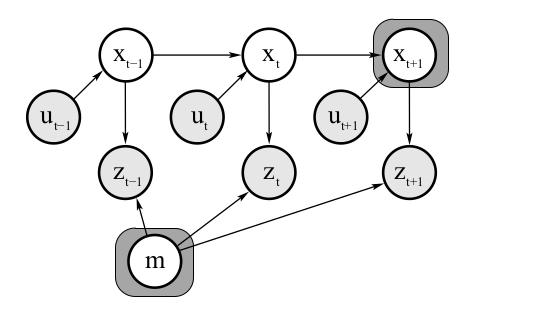
\includegraphics[width=0.9\textwidth]{images/DBN_Online.png}
        \caption{Dynamic Bayes Network for Online SLAM}
    \end{figure}
        The Pose information of the robot at time instant $t$ is represented as $x_t$ which constitues $(x,y,\theta)$.
where $(x,y)$ correspond to the location and $\theta$ represent orientation in the 2D Plane. Let $u_t$ be the Odometry reading of the motion executed between time $t-1$ and $t$. Let $Z_t$ be the LiDAR measurement
taken at time $t$. Let $m$ be the Map created from the set of measurements. In the figure \ref{fig:DBNOn}, the empty circles denote the states to be estimated and the shaded circles denote the variables that can be 
measured.Considering the circles to be the nodes and the arrows as edges, It is seen that the previous information on the state and the present command determines the current state of the system, which then influences the 
measurements obtained from the map.The nodes $m$ and $x_t+1$ are the required output parameters. There are three basic fundamental approaches to the SLAM problem, namely, \textit{Kalman Filter},\textit{Particle Filter},
\textit{Graph Network}.Each approach to the problem have their specific advantages and disavantages, which will be discussed briefly in this chapter and extensively in upcoming chapters.
 However all the methods address the basic problem -
Given the relative distance moved as recorded by the odometer and the observation at the current location, the system must be able to correctly Localize and Map its environment. 
In this chapter we will also look at how the probabilistic framework helps in achieving the task in hand and also the components commonly used across all the SLAM methods.
%%%%%%%%%%%%%%%%%%%%%%%%%%%%%%%%%%%%%%%%%%%%%%%%%%%%%%%%%%%%%%%%%%%%%%%%%%%%%%%%%%%%%%%%%%%%%%%%%%%%%%%%%%%%%%
\section{Probabilistic approach to state estimation}
    In solving the Online SLAM Problem, the joint posterior distribution over the current pose and the map is the actual state of interest.
\begin{equation} \label{eq:OnlSLM}
    p(x_t, m | z_{1:t}, u_{0:t-1})
\end{equation}
whereras to solve the full slam problem, the joint posterior distribution over  all the poses the robot had traversed and the map is the actual state of interest.
\begin{equation} \label{eq:FullSLM}
    p(x_{1:t}, m | z_{1:t}, u_{0:t-1})
\end{equation}
The distributions \ref{eq:FullSLM} and \ref{eq:OnlSLM} are applicable only to the grid based mapping. For Feature-based mapping the correspondence between the landmark measured and the 
measurement needs to be established. This is a data association problem and it could be estimated as a part of the posteriror distribution.
\begin{equation} \label{CorresSLM}
    p(x_{1:t}, m, c_t | z_{1:t}, u_{0:t-1})
\end{equation}
As this work is applicable only to Grid-based mapping, Henceforth the derivations and equations are with respect to it without being mentioned explicitly.
Applying the Bayes rule to determine the joint posterior distribution 
\begin{equation} \label{eq:FullSLMc}
    p(x_{1:t}, m | z_{1:t}, u_{0:t-1}) = \alpha . p(z_t | x_t, m).\int p(x_t| x_{t-1}, u_{t-1}). p(x_{1:t-1}, m | z_{1:t-1}, u_{0:t-2}) dx_{1:t-1}
\end{equation}
\par

%EKF SLAM
However estimating the states using \ref{eq:OnlSLM} becomes computationally expensive when integrating over all the previous poses and observation. This could be overcome by use of Extended KalmanFilter under three assumptions
\textit{Feature-Based Maps} such that the number of landmarks are less , \textit{Gaussian Noise Assumption} such that the noise levels in the robot motion and perception is in limits that does not disturb the
linearization of EKF and \textit{ Positive Information} such that unseen landmarks do not influence the estimation.In many practical applications the correspondence of a landmark to the measurement is not known.
In such cases data asssociation has to be derived during runtime.In such cases, the correspondence is also estimated in the posteriror distribution as shown in \refeq{eq:FullSLMc}.

In the online SLAM process , as the robot moves through the environment, the system state vector and the covariance matrix are updated upon new measurements. 
On observing new landmarks, new state variables are added to the system state vector and the covariance matrix. The EKF involves State Prediction and Correction step for every time a new information is received.
The State Prediction and Correction steps are elaborated in subsequent sections.
However the EKF has their own limitations. First, The covariance matrix maintained by the KalmanFilter has ${O}(K^2)$, 
where K is the number of landmarks. Thus an increase in the number of the landmarks results in longer sensor updates. Second, The correspondence of the measurement and the landmarks is assumed to be known. Any wrong data association leads to 
filter divergence.  \par
%RBPF SLAM
Overcoming the problem, Rao-Blackwellized Particle Filters were used as a effective means to estimate the full posteriror distribution. Instead of working on the entire distribution, particles were sampled at random and with 
sufficient number of particles the entire distribution could be covered.Here it is possible to relax the Gaussian assumption made in the EKF SLAM ,as any 
arbitrary distribution could be modelled as the Target distribution. It basically involves steps such as Sampling, Importance Weighting, Resampling and Map Estimation.
Sampling from proposal distribution corresponds to State prediction step and Importance Weighting corresponds to State Correction steps in EKF.
More detailed discussion on RBPF is provided in the next chapter. This method is applicable to both Grid based and Feature Based mapping with fewer modifications.\par
%Graph SLAM
The third category of SLAM ...

%%%%%%%%%%%%%%%%%%%%%%%%%%%%%%%%%%%%%%%%%%%%%%%%%%%%%%%%%%%%%%%%%%%%%%%%%%%%%%%%%%%%%%%%%%%%%%%%%%%%%%%%%%%%%%

\section{State Prediction}
    State prediction is the key component in predicting the motion of the robot in case of EKF and Filter based SLAM methods, also it helps in creating the graph in front-end of graph based SLAM.
The mobile robot is assumed to be equipped with odometer which provides relative motion of the wheels between time instances and a LiDAR sensor which can preceive the environment.
Consider the Positional state of the robot $x_{t-1}$ at time $t-1$, when subject to motion command $u_{t-1}$ the robot takes a new 
positional state $x_t$. The change in the positional state of the robot can be determined by use of motion models derived from translational and rotational kinematics or by using odometers.
In equation \ref{eq:FullSLM}, the conditional density $p(x_t| x_{t-1}, u_{t-1})$ denote the state prediction part of the equation which could be replaced with appropriate motion models to predict the state of the 
robot in motion.The motion models derived will also need to factor the noise and uncertainity in its prediction, this is captured in the process noise covariance matrix. 

\subsection{Odometry Motion Models}
The odometers are basically wheel encoders which reads how much the wheels have moved through the environment on receiving the command. Hence it can only provide motion information post-the-fact,
i.e. on receiving the motion command, the robot executes the command and then the odometry information is obtained. In many practical scenarios the robot might not follow all the motion commands as 
instructed due to slippage, wear and tear or due to any external forces. Under any such circumstances the odometer 
provides much reliable information on the state of the robot. However 
in case of motion planning this behaviour is not beneficial as the pose information at the next instance is critical to create a motion plan. In such cases the kinematic model of the 
robot is used to predict the motion of the robot. 
Algorithm for state predction using odometry based motion model is very widely used in many robotics applications. Algorithms presented in the book \cite{Thrun98aprobabilistic} can be used off-the-self 
for motion estimate implementation with odometry.
On the downside, it is very common to observe drift and slippage in the odometer information and yet,it is most widely used in many robotics and indutrial applications.

\subsection{Kinematic Motion Models}
In applications such as motion planning the positional state of the robot is required to be know in advance for better planning and control. Depending on the number of tractions, dimensions of the robot the 
kinematic equations of the motion can be used to estimate the state of the system. \cite{R.Schubert} provides a detailed study on many different motion models which falls largely under the linear and curvilinear
models. Linear motion models assume only straight motions and do not take rotations into calculation, whereas the curvilinear models assume the robot takes a circular path at a constant radius only exception being 
Constant Turn  Radius and Acceleration(CTRA) which assumes that the robot follows a clothoid. The Figure \figurename{MtnMdl.png} provides the relationship and assumptions made by each of the motion models.
The experiment results prove that curvilinear models provide better performance than linear models. Further CTRA shows better tracking results than the other curvilinear models.In \cite{Polack},similar studies were made
comparing Kinematic Bicycle Model and Dynamic models with 9-DOF, It was found that the earlier models were comparable to the dynamic model at low speeds and low angular acceleration. However at higher speeds or lateral
acceleration ,the dynamic models with higher degrees of freedom were able to accurately plan the trajectory.Simplifying the soltuion to the problem and considering the theoritical  evidence in the literature, 
CTRA Motion Model is chosen as the motion model for state prediction in our task.The motion models derived are 
in continuos domain and these need to be discretized before it could be implemented on a computer. Methods such as Euler discretization or analytical methods are some of the common methods used in deriving
discrete time representation of the process model and process covariance matrix.\cite{D.Svensson} provides the
derivation of the discrete time equations for the CTRA model along with the process noise covariance modeled.  The states involved in the prediction are longitudinal position($x(t)$), lateral position($y(t)$), heading angle($\phi(t)$), speed($s(t)$),
acceleration ($a(t)$) and yaw rate ($\omega(t)$). In continuous domain the prediction function is derived and the discrete time model is derived using linearized discretization approach
The prediction equations are given by 
\begin{gather} \label{CTRA_pred_ct}
    x_{k+1}^{CTRA}
    =
    \begin{bmatrix} 
        x_k \\ y_k \\ s_k \\ \phi_k \\ a_k\\ \omega_k
    \end{bmatrix}
    +
    \begin{bmatrix} 
        \Delta x_k \\ \Delta y_k \\ a_k T \\ \omega_k T \\ 0 \\ 0
    \end{bmatrix}
    + v_k
\end{gather}
where $T$ is predicition time and $v_k \thicksim  \mathcal{N}(0,Q_{k}^{CTRA})$ is the discrete time process noise that is a zero mean Gaussian noise with covariance $Q_k^CTRA$. For the complete derivation of the prediction function and the 
process covariance matrix refer to \cite{D.Svensson}.

%%%%%%%%%%%%%%%%%%%%%%%%%%%%%%%%%%%%%%%%%%%%%%%%%%%%%%%%%%%%%%%%%%%%%%%%%%%%%%%%%%%%%%%%%%%%%%%%%%%%%%%%%%%%%%
\section{State Correction}
    The state of the system predicted using the motion models may not accurately define the state and its variance modeled using the process covariance matrix. In order to further deteremine 
the exact posterior distribution, a confidence or a correction factor is required upon the predicted state. State correction techniques help in achieving a confidence or correction factor which
helps in extracting precise information about the state predicted using the motion model. Various observation or measurement models can be chosen based on the sensor configuration present in the robot.
In equation \ref{eq:FullSLM}, the conditional density $p(z_t | x_t, m)$ denotes the state correction part of the equation which can be replaced with appropriate measurement models or even scan matching algorithms 
to estimate a state with confidence. Given the map $m$ and pose of the robot $x_t$ , the model must be able to summarise how the surrounding environment would seem to be. Numerous of research have been conducted
on robot perception systems. Sensor systems such as LiDAR, Cameras, ultrasonic, radar are commonly used in various robotic applications depending on the environmental conditions where the robot is deployed.

\subsection{Observation Models}
In case of LiDAR, it is safe to asssume that every beam is independent of each other, hence the noise parameters and the measurement errors can be individually modelled. The measurement model density can
thus be written as 
\begin{equation}
    p(z_t | x_t, m)  = \Pi_{k=1}^k  p(z_t^k | x_t, m)
\end{equation}
where  $z_t^k$ corresponds to a single laser beam. The density $p(z_t^k | x_t, m)$ can be modelled using different algorithms. Genrally it is a mixture of four distribution- Gaussian distribution at the incidence of an obstacle, 
Exponentially decaying distribution to model unexpected objects in the view of actual obstacle, uniform distribution at the maximum range of laser beam and a uniform distribution throughout the range to include all unexpected measurements.
The estimated value of the true measurement can be achieved through ray casting operations in case of beam based models or nearest neighbour function in case of likelihood fields model.
Algorithms suggested in the book \cite{Thrun98aprobabilistic} can be used off-the-shelf for estimating the ditribution.

\subsection{Scan Matching}
    With advancement in computing power and use of
LiDAR for perception it is possible to obtain more reliable results by registering two scans taken at two different relatively close poses and extract the relative poses between the two scans. 
This process of matching two scans is termed Scan Matching and it has been widely used for various applications. In other words,it the method of finding the corrrect pose of the robot within a 3 dimensional
search space which could provide the maximum value for the density $p(z_t | x_t, m)$. 
\begin{equation}
    \hat{x} _{t} = argmax_{x} p(x|m_{t-1}, z_t, x_t)
\end{equation}
\par
Unveiling the full potential of LiDAR and its robustness in creating a scan map of the environment,
LiDAR Odometry and Mapping(LOAM) was presented in \cite{ZhangS14}. In this approach only a subset of the point clouds is used to extract useful features such as planes, lines and edges which is later 
used to derive various metrics for the scan registration. In \cite{D.Hahnel}, consistent Maps were generated with the help of 2D scan matching and also were able to detect and track people
even with the help of sample based Joint Probabilistic Data association filter.
Depending on how the point cloud data is modelled existing approaches can be classified into 
global and local scan matching. In global scan matching the point cloud is considered as a whole, but in local scan matching only segments of the point cloud are matched.

Some of the local scan matching approaches include Iterative Closest Point(ICP), Normal  Distribution Transform(NDT) and Global scan matching approaches include Correlative Scan Matching(CSM)

\subsubsection{Iterative Closest Point}
    It is the most well-known widely used algorithm known for  efficient registration of given two 2D or 3D scan or point cloud data under euclidean transformation. It is the most simple and intuitive algorithm.
Provided the correspondence between the points in the point cloud and with a  approximate initial guess, ICP tries to find the optimal motion parameters - rotation $\mathcal{R}$ and translation $\mathcal{T}$ of given 
two point cloud data. In practice the correspondence is usually unknown, hence iterative procedure is followed with good intial guess. If the intial guesses are close enough ,a converging solution is obtained.
The iteration is generally stopped after certain number of iterations or if the error value reaches below a threshold. Different variants of ICP are developed such as Point-to-Point, Point-to-Plane,
Plane-to-Plane each with its pros and cons. 

\paragraph{ICP using Spectral Value Decomposition}
First proposed in \cite{KS.Arun}, the centroid of the two point cloud data are aligned and relative rotation of the two point cloud data is obtained using SVD such that the least squared error is minimized.
In simple words the squared error in the observation from two different relatively close view points need to be minimized. 
This approach results in closed form solution only when the point correspondence of two point clouds is known. Hence it is iterated over until convergence.
\par
Given the two point cloud data $p_1$ and $p_2$, where $p_2 = \mathcal{R}p_1 + \mathcal{T} + N$, find $\mathcal{R}$ and $\mathcal{T}$ such that error function
\begin{equation}
    E(\mathcal{R}, \mathcal{T}) = \frac{1}{N_{p_1}}  \Sigma_{i=1}^{N_{p_1}}\left\lVert p_2 - \mathcal{R} p_1 -\mathcal{T} \right\rVert^2 
\end{equation}
is minimized.
where $N_{p_1}$ is the number of points in the point cloud data.

It can be accomplished by taking the centroids of the point clouds $p_1$ and $p_2$ such that
\begin{equation}
    \begin{aligned}
        \mu_{p_1}&= \frac{1}{N_{p_1}} \Sigma_{i=1}^{N_{p_1}} p_{1_i}\\

        \mu_{p_2}&= \frac{1}{N_{p_2}} \Sigma_{i=1}^{N_{p_2}} p_{2_i}\\

        P_1&= p_1 - \mu_{p_1}\\
        P_2&= p_2 - \mu_{p_2}\\

        H&\triangleq  \Sigma_{i=1}^{N} P_1 P_2^T\\
    \end{aligned}
\end{equation}
Now to find the rotational component of the motion parameters $\mathcal{R}$, 
Spectral Value Decomposition can be applied on the cross covariance matrix $H$.

When the rank(H) = 3, then a unique and optimal solution for $E(\mathcal{R}, \mathcal{T})$ is obtained.
The rotational component $\mathcal{R}$ can be obtained by 
$\mathcal{R} = \mathcal{U} \mathcal{V}^T$

The translation component $\mathcal{T}$ can be obtained by 
$\mathcal{T} = \mu_{p_1} - \mathcal{R}\mu_{p_2} $

The error encountered in the process is given by 
$E(\mathcal{R}, \mathcal{T}) = \Sigma_{i=1}^{N_{p_2}}(\left\lVert x_i^{'} \right\rVert^2 + \left\lVert y_i^{'} \right\rVert^2)$ - 2* Singular values of $H$.

The approach presented above is applicable to point to point alignment and it could be modified and used for other variants of ICP. Being an iterative procedure and non-convex problem, ICP is susceptible to settle at local 
minima.This might results in non optimal solution. Methods such as GO-ICP \cite{Yang_2016} were developed for global optimal solution. It is based on Branch-and-Bound theory for global optimization and the local-ICP procedure.
It constitutes a outer loop of BnB search in the rotation space of SO(3) and then solves for optimal search in inner loop for translational space. The search for the optimal parameters then stops on reaching
a so-far-the best error threshold or the search is terminated when the search cubes are sufficiently small. 
\par
%%%%%%%%%%%%%%%%%%%%%%%%%%%%%%%%%%%%%%%%%%%%%%%%%%%%%%%%%%%%%%%%%%%%%%%%%%%%%%%%%%%%%%%%%%%%%%%%%%%%%%%
\paragraph{ICP using Gauss-Newton (Least squares approach)}
However this put restrictions on the choice of error funtion to be used ,hence a more generic approach to find solution to the prooblem is
to take least squares using Gauss-Newton method. This method also tries to minimize the error but the error function can be chosen appropriately. The error function is then linearized
using Taylor series expansion and by forming the hessian matrix and jacobian vector the desired paramters can be obtained iteratively.
Given the two point cloud data $p_1$ and $p_2$, , where $p_2 = \mathcal{R}p_1 + \mathcal{T} + N$,the error function defines how varied are the points.
Let the error function be 
    $E(\mathcal{R}, \mathcal{T}) = \Sigma_{i=1}^{N_{p_1}}\lVert p_2 -  p_1 \rVert^2 $
assuming the correspondences are known.
\par
Linearizing the above equation
    $E(\mathcal{R}+\Delta{R} , \mathcal{T}+ \Delta{T}) = E(\mathcal{R}, \mathcal{T}) + \mathcal{J}_E(\mathcal{R}, \mathcal{T})(\Delta{R} ,\Delta{T})$
    where,
    $\mathcal{J}_E(\mathcal{R}, \mathcal{T}) = \partial (E) / \partial (\mathcal{R}, \mathcal{T})$

Solving the above error equation by Gauss-Newton approach, the change in the parameters is derived as a small step towards reaching the global minimum of the error funciton.
    $\Delta(X) = -\mathcal{H}^{-1} b$
    where,
    $\mathcal{H} = \mathcal{J}_E^{T}\mathcal{J}_E$
    $b = \mathcal{J}_E^{T} E$

Since the Gauss-Newton approach takes only in steps to reach the global minima, the procedure is repeated in iterations.
\par
%%%%%%%%%%%%%%%%%%%%%%%%%%%%%%%%%%%%%%%%%%%%%%%%%%%%%%%%%%%%%%%%%%%%%%%%%%%%%%%%%%%%%%%%%%%%%%%%%%%%%
\paragraph{ICP with Point-to-Plane correspondence}
The point to point correspondence assumed in the above methods can be achieved using Neareset Neighbour algorithms. However this stratergy might lead to wrong correspondences as it is only considers the points as discrete
whereas in reality these points actually represent the hidden structure in the surrounding. Thus considering the surfaces of the obstacle would provide better correspondences, this results in Point-to-Plane matching.
\par
In the Point-to-Plane correspondence still the closest points are considered as initial guess to define the surface. Then the point to point projection of the error vector is projected on to the surface of the normal of the 
target scan. This process is repeated until the projection of error vector on the normal is minimal.
The Point-to-Plane correspondence can be used along with Gauss-Newton approach to get better results.
Further the robustness of the ICP algorithms can be enhanced by rejecting the outliers in the point cloud data such as dynamic obstacles and reflections.

\subsubsection{Real-Time Correlative Scan Matching}
    Perhaps the most efficient, intuitive and robust method commonly used in almost all modern day robot for scan matching is the Real-Time Correlative Scan Matching proposed by E.Olson in \cite{E.B.Olson} inspired from \cite{Konolige} 
correlation based localization. It provides a novel multi-resolution approaches to compute the motion parameters in conventional CPUs and modern day GPUs. It is based upon cross correlation fo two lidar scans through 
probabilistic approach. It finds the rigid body transformation that maximizes the probability of having observed a scan instead of using a local search algorithm to find global maximum. The efficient computation of the density
$p(z_t | x_t, m)$ is made possible by implementing a multi-level resolution of the rasterized cost map. First a low-resolution cost map is used to find the area of the global maximum with the position of the robot
established predicted by the motion model. This ensures that search volume in high resolution is reduced. With the region of global maximum observed, the search is repeasted with the high-resolution 
cost map. This method proves to be exceptionally robust and it is been widely used in the industry and many open source SLAM implementations like cartographer. 
    This method has an advantage that it not only computes the motion parameters, but it tries to compute the entire density $p(z_t | x_t, m)$, hence uncertainity of the estimated motion paramters is also calculated.
    Based on \cite{E.Olson}, a similar multi-resolution approach is proposed with increased accuracy and better quality in \cite{P.Vath}. In this the author uses not only the occupied cells but also the unoccupied cells for scoring the 
scan match based on the choice of pose in the 3D search space.The score function adds up positively in case of matching occupied cells and negatively for mismatching unoccupied cells.

\subsubsection*{Normal Distribution Transform}
    \cite{P.Biber} proposed a alternative method for matching lidar scans using normal distributions to cells in a local map that can be used to match another normal distributed cells in a map using Newton's optimization 
algorithm. The Occupancy grid created around the robot is discreted into cells of appropriate size and a normal distribution is formed for the cells which contain more than 3 detections in it.Now a 2D plane in 
the form of probability distribution is achieved. In order to minimize discretization effects, maps which are shifted by all 4 directions are overlapped to get a continous distribution.
    In order to match two given scans, the NDT of the first scan is created and with the predicted motion parameters, the second scan points are mapped into the coordinate frame of first 
scan and the normal distribution is constructed for each matched point. The score for the parameters is determined by evaluating the distribution and summing the result. This is then optimized using
Newton's equation and repeated until the convergence is met. Since only the distribution of the detections is considered,It is proven to be faster than ICP.
 The algorithm is proven to work efficient for SLAM and position tracking.
    Similar approach was taken by \cite{K.Ryu} in which new scans were matched to previous scan by ICP but are later corrects the error by matching to globally defined map. The global map is constructed as a
Normal Distribution and the new scan is matched to the NDs for correcting the errors.Thus it performs a ND-to-ND matching using Kullback-Leibler (KL) divergence.
The author claims that this methods has the benefits of both ICP and NDT
\par
\cite{HaoFU} evaluated popular scan matching approaches using a LiDAR dataset recorded in off-road environment and proposed an alternative approach combining local and global  scan matching to obtain the 
best of both.

\subsubsection{Loop Closure}
In several cases the robot might traverse through a previously visited location and it must be able to recognize it and it is termed as \textit{loop closing}. This enables to 
achieve better accuracy of the Map.Apart from Map building the ability of robots to recognize the previously visited place or learned location enables the bot to fallback to 
the specific location in use cases such as trouble shooting, charging dock and determining desttination. 
The problem of Loop closure is challenging as in the real world the algorithm must be able to achieve good results even in dynamic environment. Also the robot must be capable 
of identifying similar looking environment. This method of relating the current measurement with a previous measurement is a process of \textit{data association}. Errors are 
common in \textit{data association} and it leads to divergence of the map when the errors in \textit{data association} are not handled carefully.With the presence of landmarks 
the covariance information of the landmarks is required.
\cite{E.Olson/LocalSM} poposed methods to determine whetehr a local scan match is globally correct. It also incorporates ambiguity and outlier testing using 
\textit{Single Cluster Graph Partitioning (SCGP)}. It also argues that the amount of evidence to determine the similarity between two places scales with robots positional uncertainity.
Find Local matches withon a seacrch afea provided by a prior , then combine multiple scans to get a latger local matches.
In order to estimate the relative positional uncertainity between nodes a and b, the determinant of the covariance matrix provides the search space to find the pose b from pose a.
Using Dijkstra projection algorithm, the uncertainity is estimated and the relative uncertainity between two paths is dominated by the shortest one. 

Grouping
pairwiseconsistncy
local uniqeness and oyutlier rejection
global sufficiency

Apart from SGCP methods such as Combined Constraint Data Association, Joint Compatability Branch and Bound and Cyclic verification of cumulative transformations are also available
to remove false positive loop closures.However the performance of these methods depens on good initialization \cite{P.Agarwal}.
%%%%%%%%%%%%%%%%%%%%%%%%%%%%%%%%%%%%%%%%%%%%%%%%%%%%%%%%%%%%%%%%%%%%%%%%%%%%%%%%%%%%%%%%%%%%%%%%%%%%%%%%%%%%%%
\section{Summary}